\documentclass{bschlangaul-aufgabe}
\bLadePakete{mathe,grafik}
\begin{document}
\bAufgabenMetadaten{
  Titel = {Aufgabe 5},
  Thematik = {Transaktionen T1 und T2},
  Referenz = 66116-2021-F.T1-TA2-A5,
  RelativerPfad = Staatsexamen/66116/2021/03/Thema-1/Teilaufgabe-2/Aufgabe-5.tex,
  ZitatSchluessel = examen:66116:2021:03,
  BearbeitungsStand = mit Lösung,
  Korrektheit = unbekannt,
  Ueberprueft = {unbekannt},
  Stichwoerter = {Transaktionen},
  EinzelpruefungsNr = 66116,
  Jahr = 2021,
  Monat = 03,
  ThemaNr = 1,
  TeilaufgabeNr = 2,
  AufgabeNr = 5,
}

Gegeben sind die folgenden transaktionsähnlichen Abläufe. (Zunächst wird
auf das Setzen von Sperren verzichtet.) Hierbei steht R(X) für ein
Lesezugriff auf X und W(X) für einen Schreibzugriff auf X.
\index{Transaktionen}
\footcite{examen:66116:2021:03}

\begin{center}
\begin{tabular}{|l|l|}
\hline
T1        & T2 \\\hline
R(A)      & R(D) \\
A := A-10 & D := D-20 \\
W(A)      & W(D) \\
R(C)      & R(A) \\
R(B)      & A := A+20 \\
B := B+10 & W(A) \\
W(B)      &
\\\hline
\end{tabular}
\end{center}

\noindent
Betrachten Sie folgenden Schedule:

\begin{center}
\begin{tabular}{|l|l|}
\hline
T1        & T2 \\\hline
R(A)      & \\
          & R(D) \\
          & D := D-20 \\
          & W(D) \\
          & R(A) \\
          & A := A+20 \\
          & W(A) \\
A := A-10 & \\
W(A)      & \\
R(C)      & \\
R(B)      & \\
B := B+10 & \\
W(B)      & \\\hline
\end{tabular}
\end{center}

\begin{enumerate}

%%
% a)
%%

\item Geben Sie die Werte von $A$, $B$, $C$ und $D$ nach Ablauf des
Schedules an, wenn mit $A = 100$, $B = 200$, $C = \text{true}$ und $D =
150$ begonnen wird.

\begin{bAntwort}
\begin{description}
\item[A] 90 (A := A - 10 := 100 - 10) T2 schreibt 120 in A, was aber von T1 wiederüberschrieben wird.
\item[B] 210 (B wird nur in T1 gelesen, verändert und geschrieben)
\item[C] true (C wird nur in T1 gelesen)
\item[D] 130 (D wird nur in T2 gelesen, verändert und geschrieben)
\end{description}
\end{bAntwort}

%%
% b)
%%

\item Geben Sie den Dependency-Graphen des Schedules an.

\begin{bAntwort}
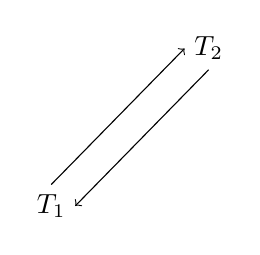
\begin{tikzpicture}
\node (T1) {$T_1$};

\node (T2) at (2,2) {$T_2$};

\draw[->] (T1.north) -- (T2.west);
\draw[->] (T2.south) -- (T1.east);
\end{tikzpicture}
\end{bAntwort}

%%
% c)
%%

\item Geben Sie alle auftretenden Konflikte an.

\begin{bAntwort}
$R_1(A) < W_2(A)$ resultierende Kante $T_1 \rightarrow T_2$,

$R_2(A) < W_1(A)$ resultierende Kante $T_2 \rightarrow T_1$,

$W_2(A) < W_1(A)$ resultierende Kante $T_2 \rightarrow T_1$ (bereits vorhanden)
\end{bAntwort}

%%
% d)
%%

\item Begründen Sie, ob der Schedule serialisierbar ist.

\begin{bAntwort}
Nicht ohne den Einsatz der Lese- und Schreibsperren, denn der Dependency
Graph enthält einen Zyklus, womit er nicht konfliktserialisierbar ist.
\end{bAntwort}

%%
% e)
%%

\item Beschreiben Sie, wie die beiden Transaktionen mit LOCK Aktionen
erweitert werden können, so dass nur noch serialisierbare Schedules
ausgeführt werden können. Die Angabe eines konkreten Schedules ist nicht
zwingend notwendig.

\begin{bAntwort}
Hier führt die Verwendung des Zwei-Phasen-Sperrpotokolls zur gewünschten
Serialisierbarkeit. (Es muss dabei weder die konservative, noch die
strenge Variante verwendet werden, damit es funktioniert). T1 würde zu
Beginn die und Lese- und Schreibsperre für A anfordern, den Wert
verändern, zurückschreiben und anschließend die Sperren für A
zurückgeben. Währendessen könnte T2 „ungestört“ die Schreib- und
Lesesperren für D anfordern, D lesen, verändern und schreiben, und die
Sperren zurückgeben. T2 bemüht sich nun um die Lesesperre für A, muss
aber nun so lange warten, bis T1 die Schreibsperre zurückgegen hat.
Dadurch kann man den Lost-Update-Fehler vermeiden und erhält allgemein
einen serialisierbaren Schedule.

Beispiel für einen konkreten Schedule mit LOCKs (auch wenn nicht
zwingend gefordert in der Aufgabenstellung):

\begin{tabular}{|l|l|}
\hline
T1             & T2                 \\\hline
rLock(A)       &                    \\
xLock(A)       &                    \\
               & rLock(D)           \\
               & xLock(D)           \\
R1(A)          &                    \\
               & R2(D)              \\
A := A-10      &                    \\
               & D := D-20          \\
               & W2(D)              \\
               & unLock(D)          \\
               & rLock(A) DELAY     \\
W1(A)          &                    \\
unLock(A)      &                    \\
               & R2(A)              \\
               & A := A+20          \\
               & W2(A)              \\
               & unLock(A)          \\
rLock(C)       &                    \\
R1(D)          &                    \\
unLock(C)      &                    \\
               & commit             \\
rLock(B)       &                    \\
xLock(B)       &                    \\
R1(B)          &                    \\
B := B+10      &                    \\
W1(B)          &                    \\
unLock(B)      &                    \\
commit         &                    \\
\hline
\end{tabular}

\end{bAntwort}

\end{enumerate}
\end{document}
